 \documentclass{exam} 
%\documentclass[answers]{exam} 
\usepackage{amsmath,amssymb,enumitem,amsthm,
%fdsymbol,
float,tikz,pgfplots,etoolbox,ifthen,xcolor,fullpage,graphicx,comment,hyperref,environ,array} 

\pgfplotsset{compat=1.17}


%%%%%%%%%%%%%%%%%%%%%%%%%%%%%%%%%%%%%%%%%%%%%%%%%%%%%%%%%%%%%%%
% Add some star options
%%%%%%%%%%%%%%%%%%%%%%%%%%%%%%%%%%%%%%%%%%%%%%%%%%%%%%%%%%%%%%%
\usetikzlibrary{shapes.geometric, calc} %testing stars...  use \starscore{numStarsFilled}{numStarsTotal} -kmp
\newcommand\starscore[2]{%
  \pgfmathsetmacro\pgfxa{#1 + 1}%
  \tikzstyle{scorestars}=[star, star points=5, star point ratio=2.5, draw, inner sep=0.12em, anchor=outer point 3]%
  \begin{tikzpicture}[baseline=2pt]
    \foreach \i in {1, ..., #2} {
      \pgfmathparse{\i<=#1 ? "black" : "white"}
      \edef\starcolor{\pgfmathresult}
      \draw (\i*1em, 0) node[name=star\i, scorestars, fill=\starcolor, semithick]  {};
    }
    \pgfmathparse{#1>int(#1) ? int(#1+1) : 0}
    \let\partstar=\pgfmathresult
    \ifnum\partstar>0
      \pgfmathsetmacro\starpart{#1-(int(#1)}
      \path [clip] ($(star\partstar.outer point 3)!(star\partstar.outer point 2)!(star\partstar.outer point 4)$) rectangle 
      ($(star\partstar.outer point 2 |- star\partstar.outer point 1)!\starpart!(star\partstar.outer point 1 -| star\partstar.outer point 5)$);
      \fill (\partstar*1em, 0) node[scorestars, fill=black]  {};
    \fi
  \end{tikzpicture}%
}

\usepackage[normalem]{ulem}
\addpoints
\marksnotpoints

\definecolor{MyGreen}{rgb}{0.1, 0.4, 0.1}
\definecolor{MyBlue}{rgb}{0.1, 0.1, 0.9}

\AtBeginEnvironment{solution}{\color{MyGreen}}

\newboolean{NoSolutions} 
% Select one of the following two active lines.
% (The \setboolean command allows you to use ifthen)
%\noprintanswers\setboolean{NoSolutions}{true}
\printanswers  \setboolean{NoSolutions}{false}

%Add rubrics
\usepackage{tagging}
% Comment out this line to hide the rubric text:
\usetag{rubric}

\newcommand\pts[1][2]{\textcolor{MyBlue}{\text{\bf [#1 pts]}}}
\newcommand\pt{\textcolor{MyBlue}{\text{\bf [1 pt]}}}

\newcommand\rubric[1]{\tagged{rubric}{\textcolor{MyBlue}{#1}}}

\newenvironment{rubricEnv}{\taggedblock{rubric} \color{MyBlue}}{\endtaggedblock}

\newcommand{\onestar}{\raisebox{0.05cm}{\resizebox{1.6cm}{!}{$\bigstar\largewhitestar\largewhitestar\largewhitestar$ \ }}}
\newcommand{\twostar}{\raisebox{0.05cm}{\resizebox{1.6cm}{!}{$\bigstar\bigstar\largewhitestar\largewhitestar$ \ }}}
\newcommand{\threestar}{\raisebox{0.05cm}{\resizebox{1.6cm}{!}{$\bigstar\bigstar\bigstar\largewhitestar$ \ }}}
\newcommand{\fourstar}{\raisebox{0.05cm}{\resizebox{1.6cm}{!}{$\bigstar\bigstar\bigstar\bigstar$ \ }}}

\newcommand{\lr}[3]{\left#1{\mathstrut#3}\right#2}
\newcommand{\abs}[1]{\lr\vert\vert{#1}}
\renewcommand{\half}{\frac{\textstyle 1}{\textstyle 2}}
\renewcommand{\o}{\omega}
\renewcommand{\a}{\alpha}
\renewcommand{\b}{\beta}
\renewcommand{\bar}[1]{\mskip.5\thinmuskip\overline{\mskip-.5\thinmuskip {#1} \mskip-.5\thinmuskip}\mskip.5\thinmuskip}


\everymath{\displaystyle}
\newcommand{\diff}[2]{\frac{\text{d}#1}{\text{d}#2}}


\begin{document}

\subsection*{MATH 101A --- ASSIGNMENT 2}

\subsubsection*{Learning goals}
\begin{itemize}
    \setlength\itemsep{0.1em}
    \item Calculate volumes of revolution by the disk method (review).
    \item Calculate volumes of revolution by the method of cylindrical shells.
    \item Calculate solid volumes by slicing.
    \item Evaluate the Gaussian Integral, $\displaystyle I = \int_{-\infty}^{\infty} e^{-x^2}\,dx$.
\end{itemize}

\subsubsection*{Contributors}

\textit{On the first page of your submission, list the student numbers and full names (with the last name in \textbf{bold}) of all team members. Indicate members who have not contributed using the comment ``(non-contributing)''.}

\begin{itemize}
    \item \#00000000 Randy {\bf Zhu}
\end{itemize}

\subsubsection*{Reflection question}

\textit{Reflection questions encourage you to think about how mathematics is done. This is an important ingredient of success. Reflection questions contribute to your \textbf{engagement grade}.}

\begin{questions}

\question In written assignments you are asked to solve difficult problems as a team. 
Understanding how to approach or begin a problem is often the most
challenging aspect of problem solving. 
Discuss the following prompts together and
write a one or two paragraph response addressing all three.

\begin{parts}
    \part What strategies
does your team use when you are stuck and do not know how to approach or begin
to solve a problem?

\part Which strategies have you found to be the most effective?

\part Is the way you approach difficult problems in math similar to how you approach
difficult problems in other subject areas? Explain why or why not.
\end{parts}

\begin{solution}
    When we don't understand how to approach a problem, we try to restrict the problem to a smaller sub-problem, perhaps specializing a variable with a substituted value. We also bounce ideas around as a team. Another strategy is simply just waiting, taking a break, doing something else like going outside for a walk, instead of bashing one's proverbial head against a proverbial wall. Looking at Piazza for tips given out by fellow students, TAs, and instructors was also incredibly helpful, but in a way spoiled the learning process.

    While restricting the problem to smaller sub-problems generally helps for proving things in computer science courses, we mostly struggled with the algebra in \ref{coneSliceAntiderivative}, which couldn't really be specialized. Piazza was incredibly helpful and so was going outside and taking a break, and re-approaching the problem with a fresh perspective.

    Solving problems in this course is indeed similar to solving difficult problems in other subject areas, especially quantitative ones. But the basic principle of breaking down problems into bite-sized sub-problems that you won't choke on applies for almost any problem in life.
\end{solution}

\end{questions}
%\vfill\clearpage

\subsubsection*{Assignment questions: Three Volumes, Three Ways}

\noindent
\textit{The questions in this section contribute to your \textbf{assignment grade}.
Stars indicate the difficulty of the questions, as described on Canvas.}

\smallskip
\noindent
\textit{Before starting work on this assignment,
please read through all the questions and take note
of the special instructions in the section headed
``Notes and Comments'' below.}


\bigskip

\noindent
For any positive-valued function $r$ and interval $[z_0,z_1]$, the equation
\[
x^2 + y^2 = r(z)^2,\qquad z_0\le z\le z_1
\]
describes a 3D surface for which the horizontal slice at level $z=c$
consists of points $(x,y,z)$ where $x^2+y^2=r(c)^2$ and, of course, $z=c$.
(The informal phrase ``flying circle'' could be used.)
Textbooks call shapes like this ``surfaces of revolution'',
because they can be produced by revolving a curve in the $xz$-plane
(where $y=0$) around the $z$-axis.
The curve is defined by the pair of equations $y=0$ and $x=r(z)$.
Here is an example, in which $[z_0,z_1]=[0,2\pi]$ and $r(z) = \sqrt{(2+\cos^2(2z))}/3$.
\[
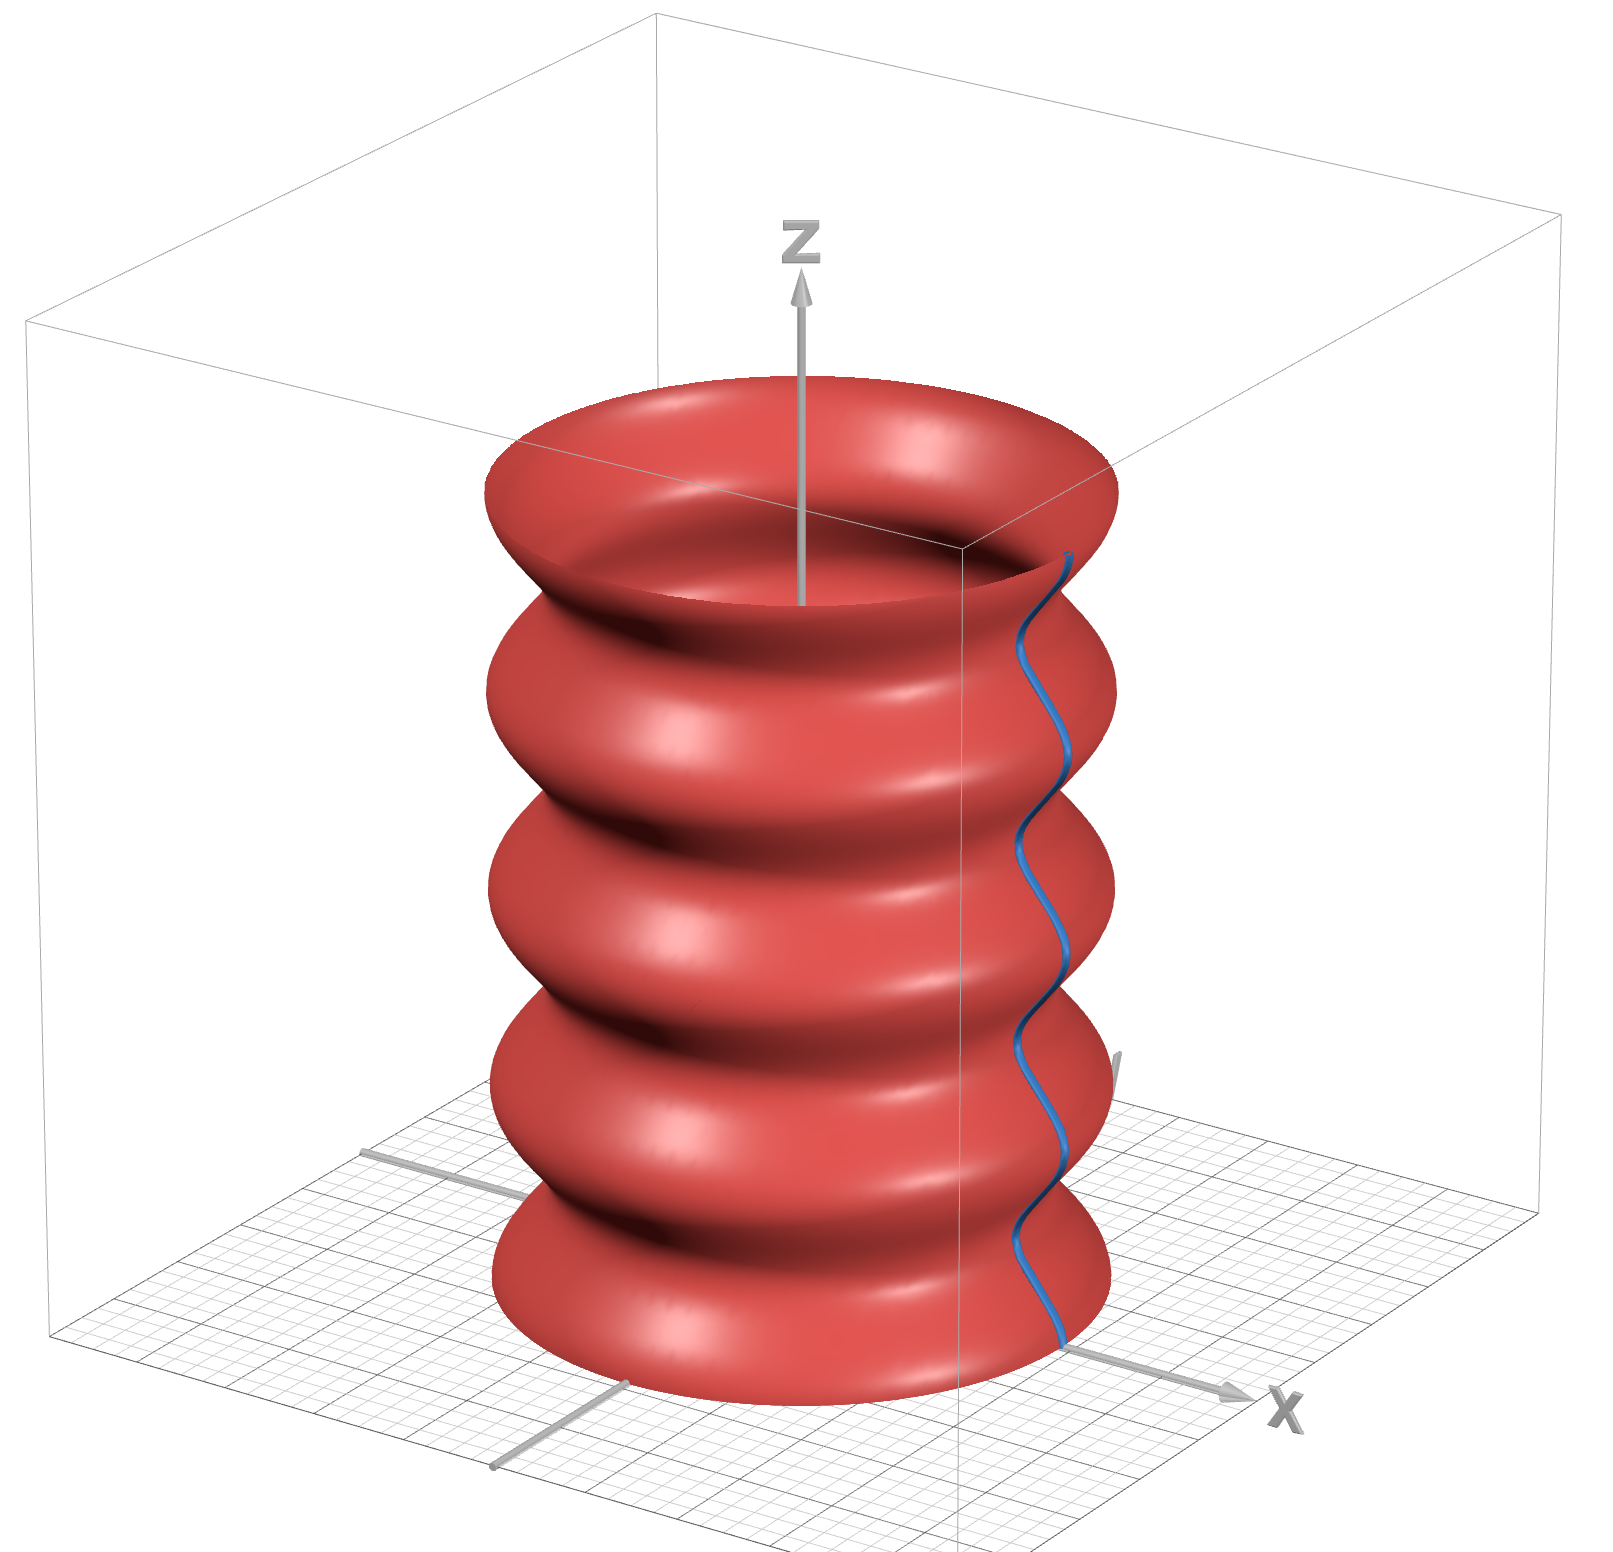
\includegraphics[scale=0.12]{kongtoy.png}
\]
This assignment considers 3 idealized shapes whose sides
are surfaces of revolution resembling real objects:
the cone, the skep, and the bump.
\[
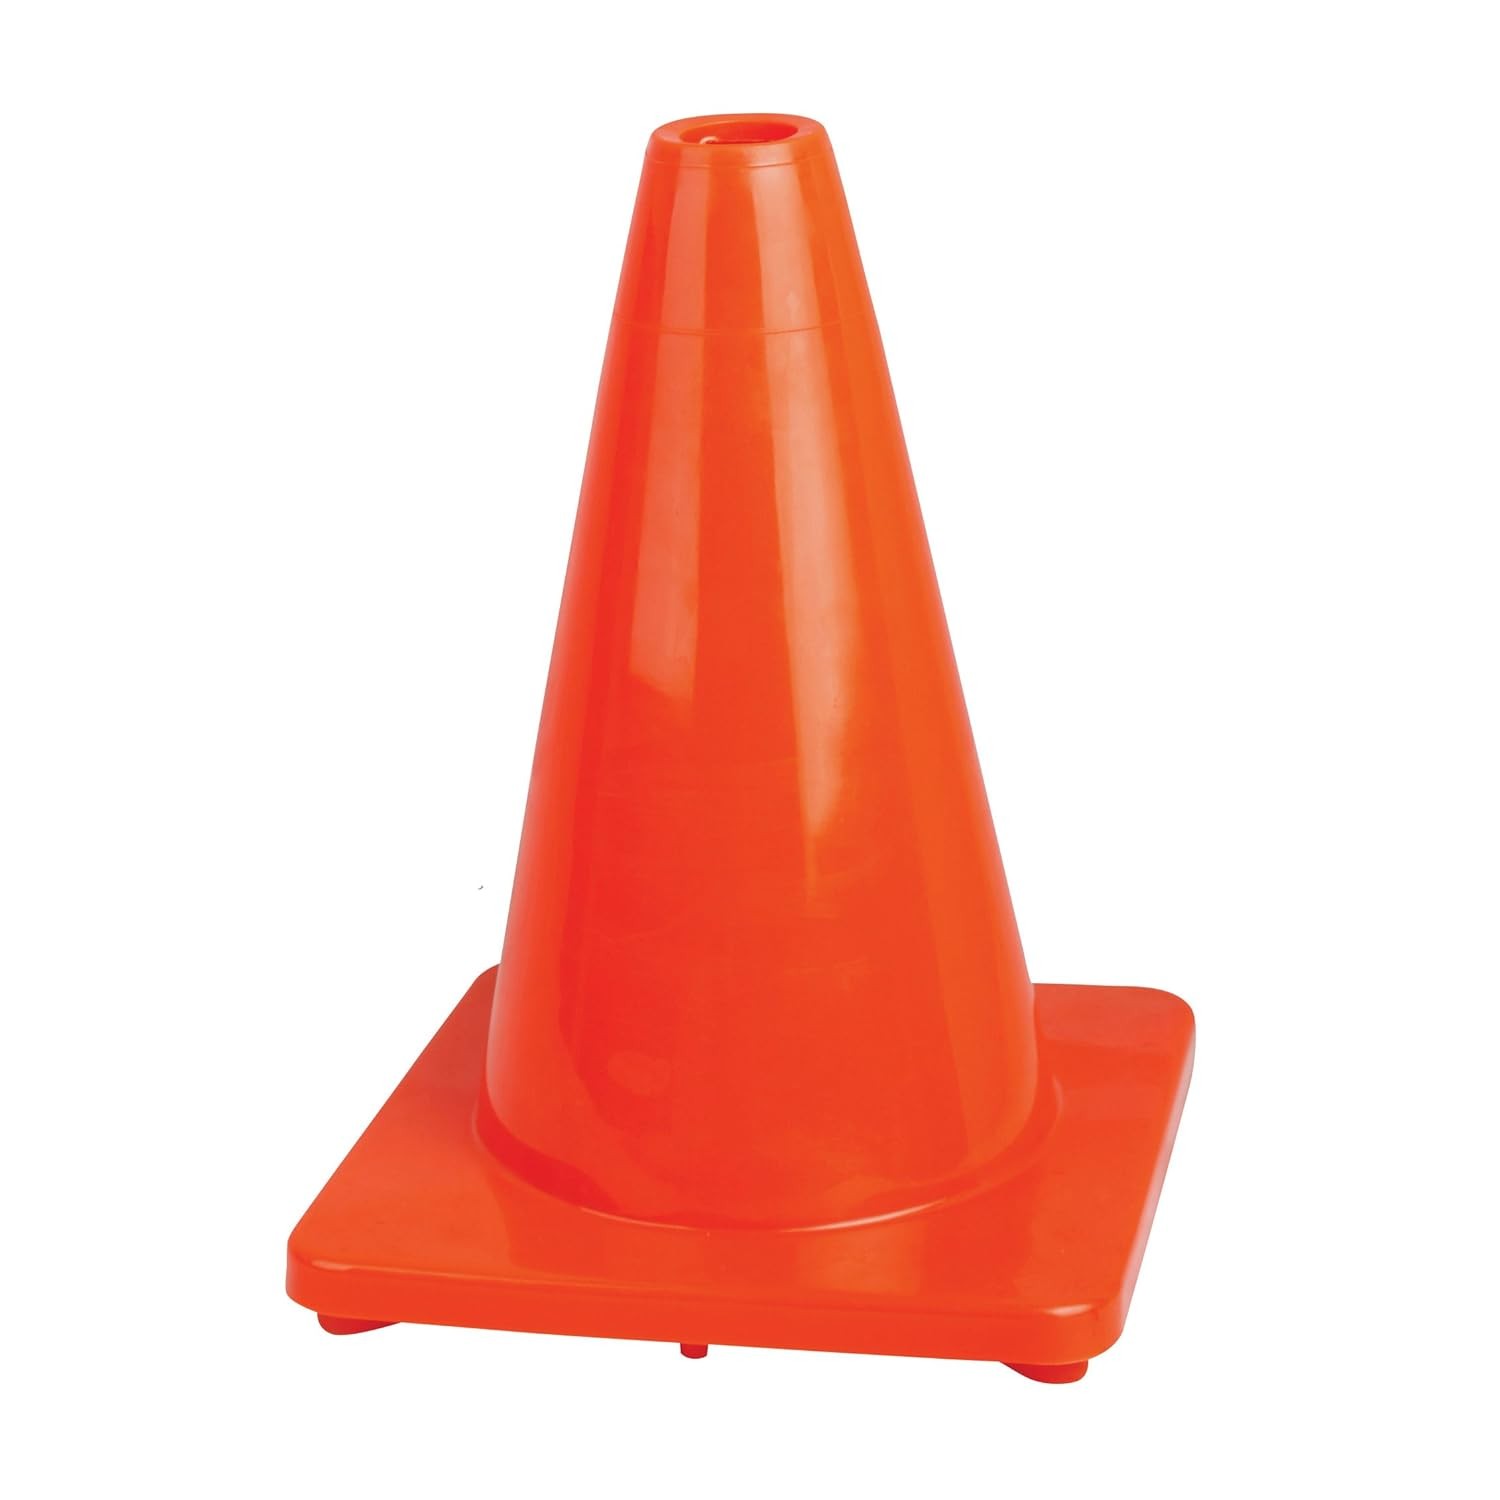
\includegraphics[scale=0.08]{cone.jpg}
\quad
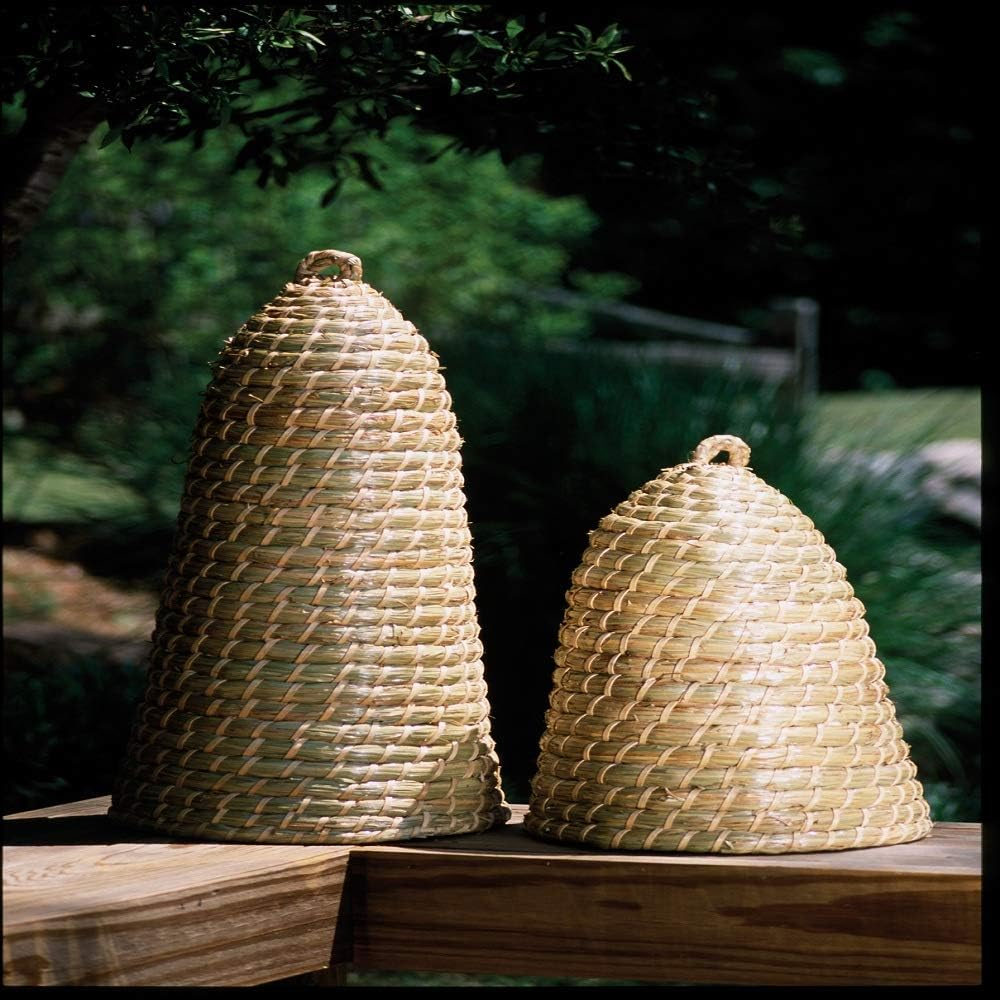
\includegraphics[scale=0.12]{skep.jpg}
\quad
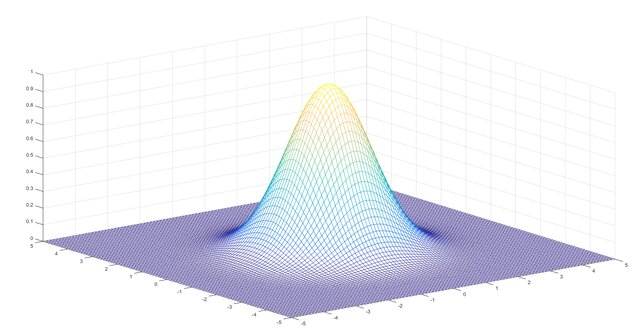
\includegraphics[scale=0.30]{bump.jpg}
\]
We can make these by spinning curves with the special
form $z=f(x)$, $y=0$, where $r_0\le x\le r_1$ and $r_0\ge0$.
Spinning any point $(x,0,z)$ around the $z$-axis will produce a flying
circle at height $z$ with radius $x$.
Algebraically, replacing $x$ with $r=\sqrt{x^2+y^2}$
upgrades the curve just mentioned into the following
3D equation defining the surface of revolution:
\[
z = f(r),\quad r_0\le r\le r_1;
\qquad r=\sqrt{x^2+y^2}.
\]
(Notice how substituting $y=0$ recovers $r=x$ and produces the original curve.)
% (Note that the earlier sketch cannot be captured in the latter form.)

\goodbreak

\noindent
For each of these solids, 
we will complete and compare three approaches to finding the volume:
\begin{itemize}
\item the pile-of-disks interpretation discussed in Small Class 4;
\item the method of cylindrical shells, explained in the CLP-2 textbook, Example~1.6.9;
\item the slicing idea illustrated in CLP-2 Example~1.6.6, in which
the volume of any solid is given by
\[
V = \int_{x_0}^{x_1} A(x)\,dx,
\]
where $A(x)$ is the area of the cross-section of the solid in the
plane perpendicular to the $x$-axis at the named point $x$,
and the limits of integration correspond to the exact interval 
$x_0< x< x_1$
in which $A(x)>0$.
\end{itemize}

\noindent
(The pile-of-disks approach is actually a special case of the
slicing method, built using slices perpendicular to the $z$-axis.
Question~2 shows the profound difference that a wise choice of axis 
can make to the intensity of calculations required for the same result.)

\begin{questions}\setcounter{question}{1} 

\question[9]
Consider the solid circular cone with base radius $a>0$
and height $h>0$ formed by joining each point $(x,y,0)$
where $x^2+y^2\le a^2$ to the vertex $(0,0,h)$.
The volume of this solid is well known: $V=\pi a^2 h/3$.
Prove this in three different ways, as follows.

\begin{parts}

\part \starscore14
Define a function $f$ and an interval $[r_0,r_1]$ with $r_0\ge0$
for which the cone's lateral surface in 3D has the form 
$z=f(r)$, $r_0\le r \le r_1$; $r=\sqrt{x^2+y^2}$.

\begin{solution}
    Let $f(r) = Ar + B$, since

    \[f(0) = h\]
    \[f(a) = 0\]

    We get $A = - \frac{h}{a} $ and $B =h$
    
    So we define this function as $z = f(r) = h - \frac{h}{a}r$ in interval $[0,h]$.
\end{solution}

\part \starscore14
Use the pile-of-disks interpretation to set up and
evaluate an integral for $V$.

\begin{solution}
    The function $z = f(r)$ produces the $z$-axis ``height'' as a function of $r$, the distance from the origin, however, a pile-of-disks interpretation would have us integrate the distance from the origin, which are the radii of the disks by the $z$-axis.

    So we must invert the function to get $r = -\frac{a}{h}z + a$.

    Setting up our integral, we integrate from the tip of the cone to the base, which is from $0 \to h$, of the disks formed by our inverted function.

    So we have:

    \[V = \int^{h}_{0} \pi(-\frac{a}{h}z + a)^2 \mathrm dz = \pi a^2 \int^{h}_{0} 1 - \frac{2}{h}z + \frac{1}{h^2}z^2 \mathrm dz = \pi a^2 \Big( z - \frac{1}{h}z^2 + \frac{1}{3h^2}z^3 \Big|^{h}_{0} \Big) = \frac{1}{3}\pi a^2 h.\]

    As required.
\end{solution}



\part \starscore24
Use the method of cylindrical shells to set up and
evaluate an integral for $V$.

\begin{solution}
    Each cylindrical shell in this case will have:
    \begin{itemize}
        \item radius $r$
        \item height $z = h - \frac{h}{a}r$
        \item width $\mathrm dr$.
    \end{itemize}

    Therefore the volume of each shell must be $2\pi r (h - \frac{h}{a}r) \mathrm dr$.

    Summing up all the shells from the centre of the cone to the edge, we get:

    \[  V = \int^{a}_{0} 2\pi r(h - \frac{h}{a}r) \mathrm dr = -2\pi h \int^{a}_{0} r - \frac{1}{a}r^2 \mathrm dr = 2\pi h \Big( \frac{1}{2}r^2 - \frac{1}{3a}r^3 \Big|^{a}_{0} \Big) = \frac{1}{3} \pi a^2 h.\]
\end{solution}

\begin{EnvUplevel}
\noindent
Our third approach to finding the same volume involves
slicing up the cone with planes parallel to the $z$-axis.
This calls for some heavy calculations, 
broken into parts (d)--(i) below.
To simplify this development, assume $h=1$ in all that follows.

For each fixed $x_0$, with $\abs{x_0}\le a$,
imagine slicing the solid cone of interest with a plane
perpendicular to the $x$-axis at the location $x_0$.
Let $A(x_0)$ denote the area of the slice obtained.
\end{EnvUplevel}

\part \starscore14 \label{easyTriangle}
Find $A(0)$.

\begin{solution}
    Slicing a cone at $x_0 = 0$ produces a triangle of base $2a$, and height 1. By the triangle area formula we have $A(0) = \frac{1}{2} \times 2a \times 1 = a$.
\end{solution}

\part \starscore34 \label{coneSliceAreaSetup}
For each fixed $x_0$, with $0<x_0<a$,
set up a definite integral 
% with respect to $y$
whose value equals $A(x_0)$.

\begin{solution}
    Slicing the cone at $x_0$, we are given a hyperbola of the form $1 - \frac{1}{a}\sqrt{x_0^2 + y^2}$. We need to integrate from the points where the hyperbola meets the base of the cone. The base of the cone is a circle of radius $a$, and when we are integrating at $x_0$, the points that the hyperbola touch are at $\pm \sqrt{a^2 - x_0^2}$. Hence, we need to integrate from $-\sqrt{a^2 - x_0^2}$ to $\sqrt{a^2 - x_0^2}$.

    So the definite integral that defines $A(x_0)$ is:

    \[A(x_0) = \int^{\sqrt{a^2 - x_0^2}}_{-\sqrt{a^2 - x_0^2}} 1 - \frac{1}{a}\sqrt{x_0^2 + y^2} \mathrm dy.\]
    
\end{solution}

\part \starscore34 \label{coneSliceAreas}
Show how to evaluate the integral for $A(x_0)$
in part (\ref{coneSliceAreaSetup}).
After you finish, change $x_0$ to $x$ throughout the
bottom line to obtain the slice-area function $A=A(x)$
for all $x$ with $0<\abs{x}\le a$.
% Then plot the graph of $A$ on a suitable interval.
% (For the plot, use radius $a=1$.)

\begin{solution}
        \begin{align*}
        A(x_0)  &= \int^{\sqrt{a^2 - x_0^2}}_{-\sqrt{a^2 - x_0^2}} 1 - \frac{1}{a}\sqrt{x_0^2 + y^2} \mathrm dy \\
                &= \int^{\sqrt{a^2 - x_0^2}}_{-\sqrt{a^2 - x_0^2}} 1 - \frac{1}{a} \int^{\sqrt{a^2 - x_0^2}}_{-\sqrt{a^2 - x_0^2}} \sqrt{x_0^2 + y^2} \mathrm dy \\ \intertext{By some simple geometry,}
                &= 2\sqrt{a^2 - x_0^2} - \frac{1}{a} \int^{\sqrt{a^2 - x_0^2}}_{-\sqrt{a^2 - x_0^2}} \sqrt{x_0^2 + y^2} \mathrm dy \\
                \intertext{Note how $\sqrt{x_0^2 + (-y)^2} = \sqrt{x_0^2 + (y)^2}$ which implies that $\sqrt{x_0^2 + y^2}$ is even. This means we can apply the fact that if $f$ is even, then $\int^{c}_{-c} f(x) \mathrm dx = 2 \int^{c}_{0} f(x) \mathrm dx$ to arrive at:}
                &= 2\sqrt{a^2 - x_0^2} - \frac{2}{a} \int^{\sqrt{a^2 - x_0^2}}_{0} \sqrt{x_0^2 + y^2} \mathrm dy \\
                \intertext{We perform a trigonometric substitution here. Take $y = x_0 \tan(a)$, and $\mathrm dy = x_0 \sec^2(a) \mathrm da$. By our substitution, it also follows that $a = \arctan(\frac{y}{x_0})$. Changing integration bounds using this formula for $a$ and applying the substitution, we have:}
                &= 2\sqrt{a^2 - x_0^2} - \frac{2}{a} \int^{\arctan(\frac{\sqrt{a^2 - x_0^2}}{x_0})}_{0} x_0^2 \sec^3(a) \mathrm da \\
                &= 2\sqrt{a^2 - x_0^2} - \frac{2}{a}  x_0^2 \int^{\arctan(\frac{\sqrt{a^2 - x_0^2}}{x_0})}_{0} \sec^3(a) \mathrm da \\
                &= 2\sqrt{a^2 - x_0^2} - \frac{2}{a}  x_0^2 \Big( \frac{1}{2}\sec(a)\tan(a) + \frac{1}{2}\log|\sec(a) + \tan(a)| \Big|^{\arctan(\frac{\sqrt{a^2 - x_0^2}}{x_0})}_{0} \Big) \\
                \intertext{$\frac{1}{2}\sec(0)\tan(0) + \frac{1}{2}\log|\sec(0) + \tan(0)| = 0$, and $\sec\Big(\arctan\Big(\frac{\sqrt{a^2 - x_0^2}}{x_0}\Big)\Big) = \frac{a}{x_0}$ so: }
                &= 2\sqrt{a^2 - x_0^2} - \frac{2}{a} x_0^2 \Big( \frac{1}{2}\Big(\frac{a}{x_0}\Big)\frac{\sqrt{a^2 - x_0^2}}{x_0} + \frac{1}{2} \log \abs{\frac{a}{x_0}\ + \frac{\sqrt{a^2 - x_0^2}}{x_0}} \Big) \\
                \intertext{Some algebra later...}
                &= \sqrt{a^2 - x_0^2} - \frac{x_0^2}{a}\log\Big(\Big| \frac{a + \sqrt{a^2 - x_0^2}}{x_0}\Big|\Big).
    \end{align*}

    Exchanging $x_0$ for $x$, we arrive at:

    \[ A(x) = \sqrt{a^2 - x^2} - \frac{x^2}{a}\log\Big(\abs{\frac{a + \sqrt{a^2 - x^2}}{x}}\Big).\]
\end{solution}

\part \starscore14
Taken together, parts~(\ref{easyTriangle}) and~(\ref{coneSliceAreas}) 
above define $A(x)$ for each $x$ where $\abs{x}\le a$.
Show that the function $A$ is continuous at $0$.

\begin{solution}

    Filling in where $A(x)$ is not defined with our result from \ref{easyTriangle},
    
    \[ A(x) = \begin{cases}
                \sqrt{a^2 - x^2} - \frac{x^2}{a}\log\Big(\frac{a + \sqrt{a^2 - x^2}}{x}\Big) & x \in (-a, 0) \cup (0, a) \\
                a & x = 0.
    \end{cases} \]


    Recall that $A(x)$ is continuous at $0 \iff \lim_{x \to 0} A(x) = A(0) \iff \lim_{x \to 0} A(x) = a$.

    We will show that $A$ is continuous at $0$ by showing $\lim_{x \to 0} A(x) = a$. 

    \begin{align*}
        \lim_{x \to 0} A(x) &= \lim_{x \to 0} \sqrt{a^2 - x^2} - \frac{1}{a} \lim_{x \to 0} x^2 \log\Big( \abs{\frac{a + \sqrt{a^2 - x^2}}{x}} \Big) \\
                            &= |a| - \frac{1}{a}\lim_{x \to 0} x^2 \log\Big( \abs{\frac{a + \sqrt{a^2 - x^2}}{x}} \Big) \\
                            &= |a| - \frac{1}{a} \bigg( \lim_{x \to 0} x^2{\log(\abs{a + \sqrt{a^2 - x^2})}} - \lim_{x \to 0} \frac{\log(\abs{x})}{\frac{1}{x^2}} \bigg) \\
                            &= |a| - \frac{1}{a} \bigg( 0 - \lim_{x \to 0} \frac{\log(\abs{x})}{\frac{1}{x^2}} \bigg) \\
                            \intertext{As $\lim_{x \to 0} \log(\abs{x}) = -\infty$ and $\lim_{x \to 0} \frac{1}{x^2} = \infty$, we have an indeterminate form. $\frac{1}{x^2}$ and $\log(\abs{x})$ is differentiable in a neighbourhood near $0$ and we have $\lim_{x \to 0} \frac{\frac{\mathrm d}{\mathrm dx} \log(\abs{x})}{\frac{\mathrm d}{\mathrm dx}\frac{1}{x^2}} = \lim_{x \to 0} \frac{x^{-1}}{2x^{-3}} = \lim_{x \to 0} \frac{1}{2}x^2 = 0$. By L'hopitals rule, $\lim_{x \to 0} \frac{\log(\abs{x})}{\frac{1}{x^2}} = \lim_{x \to 0} \frac{\frac{\mathrm d}{\mathrm dx} \log(\abs{x})}{\frac{\mathrm d}{\mathrm dx}\frac{1}{x^2}} = 0$.}
                            &= |a| - \frac{1}{a} \bigg( 0 - 0 \bigg) \\
                            &= |a| \\
                            \intertext{As $a$ represents the radius of the base of a cone, it can never be negative, so $|a| = a$.}
                            &= a.
    \end{align*}

    We therefore have $\lim_{x \to 0} A(x) = a = A(0)$ as required.
\end{solution}



\part \starscore34 \label{coneSliceAntiderivative}
Verify that the following function is an antiderivative for
$A(x)$:
\[
F(x) 
= \frac{a^2}3\sin^{-1}\!\lr(){\frac xa}
   + \frac{2x}{3}\sqrt{a^2-x^2}
   + \frac{x^3}{3a}\log\abs{x}
   - \frac{x^3}{3a}\log\abs{a+\sqrt{a^2-x^2}}.
\]
(\emph{Hint\/}: Finding $\int A(x)\,dx$ directly is much harder
than showing that $F(x)+C$ is correct.)

\begin{solution}
    Recall $F(x)$ is an antiderivative of $A(x)$ . $F'(x) = A(x)$.

    Let us compute $F'(x)$ and show that it is equal to $A(x)$ from \ref{coneSliceAreas}.

    \begin{align*}
        F'(x) &= \frac{\mathrm d}{\mathrm dx} [F(x)] \\
              &= \frac{a}{3\sqrt{1 - \frac{x^2}{a^2}}} + \frac{2}{3}\left(\frac{a^2 - 2x^2}{\sqrt{a^2 - x^2}} \right) + \frac{1}{a}x^2 \log\abs{x} + \frac{x^2}{3a} \\
              &  - \frac{1}{a}x^2 \log\abs{a^2 + \sqrt{a^2 - x^2}} + \frac{x^4}{3a\sqrt{a^2 - x^2}(a + \sqrt{a^2 - x^2})} \\
              \intertext{Multiplying the top \& bottom of the first term by $\sqrt{a^2}$, and with the knowledge that $a > 0$, we get: }
              &= \frac{a^2}{3\sqrt{a^2 - x^2}} + \frac{2}{3}\left(\frac{a^2 - 2x^2}{\sqrt{a^2 - x^2}} \right) + \frac{1}{a}x^2 \log\abs{x} + \frac{x^2}{3a} \\
              &  - \frac{1}{a}x^2 \log\abs{a^2 + \sqrt{a^2 - x^2}} + \frac{x^4}{3a\sqrt{a^2 - x^2}(a + \sqrt{a^2 - x^2})} \\
              \intertext{Re-arranging and using the property that $\log(x) - \log(y) = \log\left( \frac{x}{y} \right)$ and re-arranging, }
              &= \frac{a^2}{3\sqrt{a^2 - x^2}} + \frac{2}{3}\left(\frac{a^2 - 2x^2}{\sqrt{a^2 - x^2}} \right) + \frac{x^2}{3a} \\
              &  + \frac{x^4}{3a\sqrt{a^2 - x^2}(a + \sqrt{a^2 - x^2})} + \frac{x^2}{a} \log\abs{\frac{x}{a + \sqrt{a^2 - x^2}}} \\
              \intertext{We want to manipulate the logarithm using the identity $-\log(x/y) = \log(y/x)$, }
              &= \frac{a^2}{3\sqrt{a^2 - x^2}} + \frac{2}{3}\left(\frac{a^2 - 2x^2}{\sqrt{a^2 - x^2}} \right) + \frac{x^2}{3a} \\
              &  + \frac{x^4}{3a\sqrt{a^2 - x^2}(a + \sqrt{a^2 - x^2})} - \frac{x^2}{a} \log\abs{\frac{a + \sqrt{a^2 - x^2}}{x}} \\
              \intertext{Yay! Our logarithm looks the same as the one in $A(x)$! Let's factor out a $\frac{1}{3}$ and distribute some terms, }
              &= \frac{1}{3} \left(
                    \frac{a^2}{\sqrt{a^2 - x^2}} + \frac{2a^2 - 4x^2}{\sqrt{a^2 - x^2}} + \frac{x^2}{a} + \frac{x^4}{a\sqrt{a^2 - x^2}(a + \sqrt{a^2 - x^2})}
              \right) \\
              & - \frac{x^2}{a} \log\abs{\frac{a + \sqrt{a^2 - x^2}}{x}} \\
              \intertext{We're going to multiply the LCD of all the terms in the parens to merge all the terms at the top of the fraction, }
              &= \frac{1}{3} \left(
                    \frac{\left(3a^{2}-4x^{2}\right)\left(a+\sqrt{a^{2}-x^{2}}\right)a+x^{2}\sqrt{a^{2}-x^{2}}\left(a+\sqrt{a^{2}-x^{2}}\right)+x^{4}}{a\sqrt{a^{2}-x^{2}}\left(a+\sqrt{a^{2}-x^{2}}\right)}
              \right) \\
              & - \frac{x^2}{a} \log\abs{\frac{a + \sqrt{a^2 - x^2}}{x}} \\
              \intertext{Applying the distributive property and cancelling terms, finally, it fits on one line now! }
              &= \frac{a^3 - ax^2  + a^2 \sqrt{a^2 - x^2} - x^2 \sqrt{a^2 - x^2}}{\sqrt{a^{2}-x^{2}}\left(a+\sqrt{a^{2}-x^{2}}\right)} - \frac{x^2}{a} \log\abs{\frac{a + \sqrt{a^2 - x^2}}{x}} \\
              \intertext{Factoring, }
              &= \frac{a(a^2 -x^2) + \sqrt{a^2 - x^2}(a^2 - x^2)}{\sqrt{a^{2}-x^{2}}\left(a+\sqrt{a^{2}-x^{2}}\right)} - \frac{x^2}{a} \log\abs{\frac{a + \sqrt{a^2 - x^2}}{x}} \\
              &= \frac{(a^2 - x^2)(a + \sqrt{a^2 - x^2})}{(a^{2}-x^{2})^{\frac{1}{2}} \left(a+\sqrt{a^{2}-x^{2}}\right)} - \frac{x^2}{a} \log\abs{\frac{a + \sqrt{a^2 - x^2}}{x}} \\
              \intertext{Cancelling terms, we arrive at: }
              &= \sqrt{a^2 - x^2} - \frac{x^2}{a} \log \abs{
                \frac{a + \sqrt{a^2 - x^2}}{x}
              } \\
              &= A(x).
    \end{align*}

    As required.
\end{solution}


\part \starscore14
Use the results from parts~(\ref{coneSliceAreas}) and~(\ref{coneSliceAntiderivative})
to evaluate the cone's volume by slicing, i.e., find $V=\int_{-a}^a A(x)\,dx$.

\begin{solution}
    By FTC2,
    \[ V = \int^{a}_{-a} A(x) \mathrm dx = F(x) \Big|^{a}_{-a} = F(a) - F(-a). \]

    Let us find $F(a)$ and $F(-a)$.

    \[ F(a) = \frac{a^2}3\sin^{-1}\!\lr(){\frac aa}
   + \frac{2a}{3}\sqrt{a^2-a^2}
   + \frac{a^3}{3a}\log\abs{a}
   - \frac{a^3}{3a}\log\abs{a+\sqrt{a^2-a^2}} = \frac{a^2}{3} \times \frac{\pi}{2}. \]
    % \bigskip

    % \\
    
    \[
        \begin{aligned}
        F(-a) = {} &\frac{a^2}3\sin^{-1}\!\lr(){\frac {(-a)}{a}} \\
                    &+ \frac{2(-a)}{3}\sqrt{a^2-(-a)^2} \\
                    &+ \frac{(-a)^3}{3a}\log\abs{(-a)} \\
                    &- \frac{(-a)^3}{3a}\log\abs{a+\sqrt{a^2-(-a)^2}} \\
                    &= \frac{a^2}{3} \times -\frac{\pi}{2}.
        \end{aligned}
    \]

    Therefore, $V = F(a) - F(-a) = \frac{a^2}{3} \times \frac{\pi}{2} - \frac{a^2}{3} \times - \frac{\pi}{2} = \frac{a^2}{3}\pi$.

    Using the known formula for a cone of base radius $a$, and height $1$, we have $V = \frac{a^2}{3}\pi$. This indeed aligns with our (tedious) $x$-axis slicing method. 
    
\end{solution}



\end{parts}

\goodbreak 

\question[4]
Let $V$ denote the volume of the 3D solid where 
$0 \le z \le h(a^2 - x^2 - y^2)/a^2$,
taking $a$ and $h$ as given parameters.
Find $V$ in three different ways, as follows:

\begin{parts}
\part \starscore14
Describe and sketch the solid object of interest.

\begin{solution}

    Observe a plot of the solid defined by $0 \le z \le h(a^2 - x^2 - y^2)/a^2$.
    
    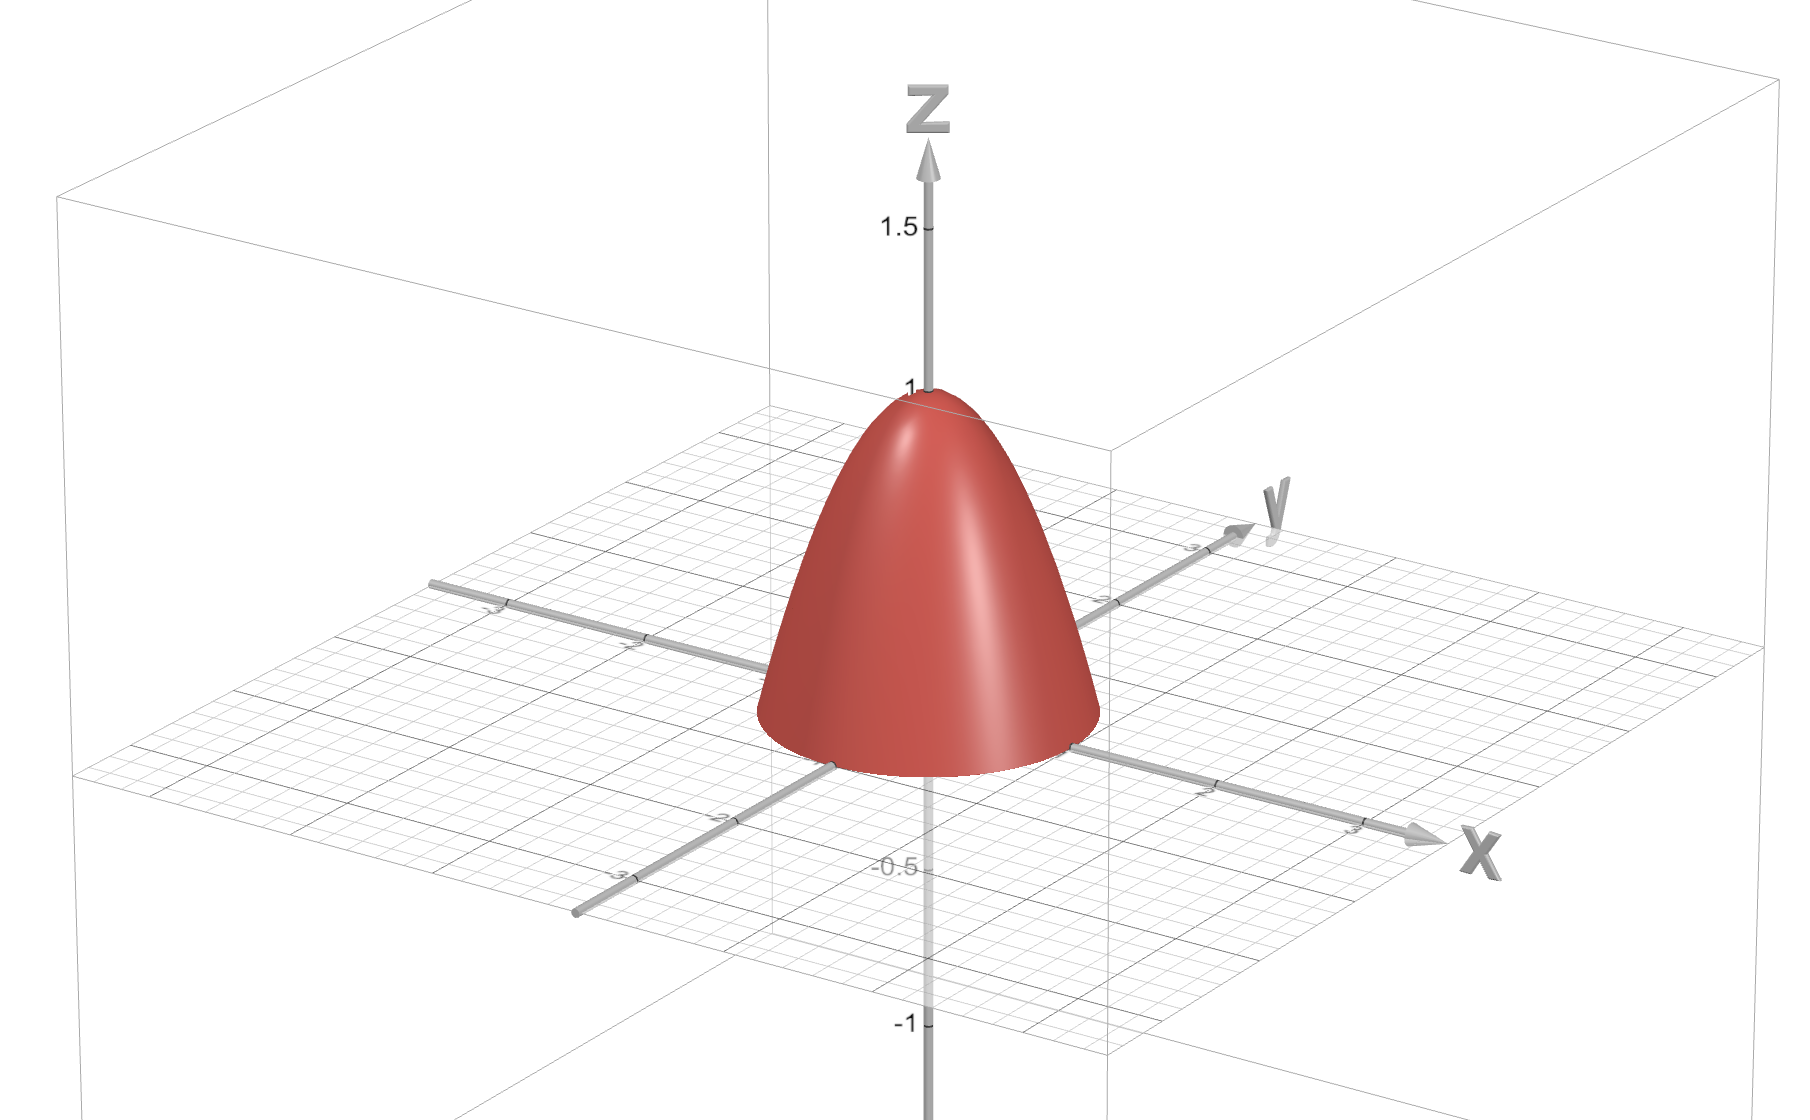
\includegraphics[scale=0.25]{image.png}

    One can describe it as perhaps a ``smooth cone''. It's essentially what happens when you rotate a filled-in parabola above $y = 0$ of the form $y = -\frac{h}{a^2}x^2 + h$ around its axis of symmetry (which in this case is just $x = 0$).
    
\end{solution}

\part \starscore14
Find $V$ using the pile-of-disks interpretation.

\begin{solution}
    We want a function that relates the square $x$ (or $y$, as this shape is symmetric about either $x$ or $y$) value to the value of $z$, as we want disks of radius $x$. We will fix $y = 0$, and this gives us:

    \[ z = h - \frac{h}{a^2}x^2. \iff x^2 = \frac{-a^2}{h}z + a^2. \]

    

    This gives us a disk of the form $\pi x^2 = \pi \left( \frac{-a^2}{h}z + a^2 \right)$.

    We integrate from $z = h$ to $z = 0$ to get:

    \[ V = \int^{h}_{0} \pi \left( \frac{-a^2}{h}z + a^2 \right) \mathrm dz = \pi a^2 \int^{h}_{0}  \left( 1 - \frac{1}{h}z \right) \mathrm dz = \pi a^2 \left( z - \frac{1}{2h}z^2 \Big|^{h}_{0} \right) = \frac{1}{2}\pi a^2 h. \]
\end{solution}


\part \starscore24
Find $V$ using the method of cylindrical shells.

\begin{solution}
    Each cylindrical shell has:
    \begin{itemize}
        \item radius $x$,
        \item height $z = h \left(1 - \frac{1}{a^2}x^2\right)$,
        \item width: $\mathrm dx$.
    \end{itemize}

    Each shell will have volume $2\pi x h \left( 1 - \frac{1}{a^2}x^2 \right) \mathrm dz$.

    Therefore:

    \[ V = \int^{a}_{0} 2\pi h x \left( 1 - \frac{1}{a^2}x^2 \right) \mathrm dx = 2\pi h \left( \frac{1}{2}x^2 - \frac{1}{4a^2}x^4 \Big|^{a}_{0} \right) = \frac{1}{2}\pi a^2 h. \]
\end{solution}

\part \starscore24
Find $V$ by considering slices perpendicular to
the $x$-axis.

\begin{solution}
    Using a similar method to \ref{coneSliceAreaSetup}, we have to fix $x$, in the same strategy, and integrate w.r.t $y$. Similarly, the circle at the base of the shape has radius $a$, and so to find where the slice of the shape, we have to integrate from $y = -\sqrt{a^2 - x^2}$ to $y = \sqrt{a^2 - x^2}$. Therefore, the function that describes the area of one single slice is the definite integral below:

    \[ A(x) = \int^{\sqrt{a^2 - x^2}}_{-\sqrt{a^2 - x^2}} \frac{h(a^2 - x^2 - y^2)}{a^2}\mathrm dy = \frac{4h(a^2 - x^2)^{\frac{3}{2}}}{3a^{2}}. \]

    Now we integrate the slices defined by $A(x)$ along the $x$-axis from $-a$ to $a$ to get the area of the shape.

    \[ V = \int^{a}_{-a} A(x) = \frac{4h}{3a^2} \int^{a}_{-a} (\sqrt{a^2 - x^2})^3 \mathrm dx =  \frac{1}{2}\pi a^2 h. \]

    All three parts converge to the same answer, surely we can't be wrong! Surely...
\end{solution}

\end{parts}

\begin{EnvUplevel}
\noindent
Some of the integrals in the next question are ``improper''.
We will study these more thoroughly later in the course.
For an operational preview, simply rely on the equations below
whenever the symbol on the left does not fit our usual situations:
\[
\int_a^b f(x)\,dx = \lim_{\alpha\searrow a} \int_\a^b f(x)\,dx,
\qquad
\int_a^b f(x)\,dx = \lim_{\beta\nearrow b} \int_a^{\b} f(x)\,dx.
\]
Whenever $f$ happens to be integrable on $[a,b]$, 
these equations are valid but uninformative.
But when $a=-\infty$ or $b=+\infty$ or the integrand is
unbounded near one of $a$ or $b$,
we can use the expressions on the right as \textit{definitions}
for the symbols on the left---provided the indicated limits exist. 
Identifying situations when all this works will be a key topic
later in the course.
In this exercise, however, all the necessary limits
can be handled by methods from a prerequisite course.
\end{EnvUplevel}

\question[4]
Let $V$ denote the volume of the 3D solid where 
$0 \le z \le e^{-(x^2+y^2)}$.
This is the infinite object above the plane $z=0$
and below the bump sketched in the introduction.

\begin{parts}

\part \starscore24
Find $V$ using the pile-of-disks interpretation.
(Consider only disks with $z>0$; 
use an improper integral as suggested above.)

\begin{solution}
    We need to transform $z = e^{-(x^2 + y^2)}$ to get a function that relates the square of $x$ (or $y$, as our shape is symmetric, but we will go with $x$) of $z$. First we fix $y = 0$ to get disks around the origin. We get $x^2 = -\log(z)$.

    Therefore, each disk has area $\pi x^2 = -\pi \log(z)$. The maximum of this shape is at $z = 1$, so we integrate from $0$ to $1$.

    Thus:

    \[ V = \int^{1}_{0} -\pi \log(z) \mathrm dz = -\pi \lim_{x \to 0^+} \int^{1}_{x} \log(z) \mathrm dz = -\pi \left( 1 \log(1) - 1 - \lim_{x\to0^+} [x\log(x) - x] \right) = \pi \]
\end{solution}

\part \starscore14
Find $V$ using the method of cylindrical shells.

\begin{solution}
    Again fixing $y=0$, we get $z = e^{-x^2}$.

    This means we have a cylindrical shell of:

    \begin{itemize}
        \item height $z = e^{-x^2}$
        \item width $\mathrm dx$
        \item radius $x$.
    \end{itemize}

    Each shell has volume $2\pi xe^{-x^2}\mathrm dz$.

    As this shape spans infinitely across the $xy$-plane, the volume is represented by:

    \[ V = \int^{\infty}_{0} 2\pi x e^{-x^2}\mathrm dx = 2\pi \lim_{t \to \infty} \Big[ \int^{t}_{0} xe^{-x^2} \mathrm dx \Big] = 2\pi \left( -\frac{1}{2} \lim_{t \to \infty} [e^{-t^2}] + \frac{1}{2}e^0 \right) = \pi \]
\end{solution}





\part \starscore34
Define $I=\int_{-\infty}^\infty e^{-u^2}\,du$.
This is a positive number whose exact value we intend to discover.
Use slices perpendicular to the $x$-axis\
to find an equation relating $V$ to $I$.

\begin{solution}
    Let $A(x)$ be some function that produces the area of a slice of the shape at some $x$ coordinate. It's defined by $\int^{\infty}_{-\infty} e^{-(x^2 + y^2)} \mathrm dy$. We can manipulate it into $e^{-x^2} \int^{\infty}_{-\infty} e^{-y^2} \mathrm dy$. By the definition of $I$, we therefore have $A(x) = Ie^{-x^2}$. Note that $I$ is wholly a function of $y$ and not $x$.

    $V$ is defined by $\int^{\infty}_{-\infty} A(x) \mathrm dx$. Therefore we have:

    \[ V = \int^{\infty}_{-\infty} A(x) \mathrm dx = I \int^{\infty}_{-\infty} e^{-x^2} \mathrm dx = I^2 ~\text{by definition of } I. \]
\end{solution}


\part \starscore14
Determine the exact value of $I$.
(This is an important constant worth remembering.)

\begin{solution}
    $V = I^2 = \pi$ which means $I = \sqrt{\pi}$. Note that because $e^{-u^2}$ is always positive so $I$ must always be positive, so we discard the negative solution for $I$.
\end{solution}



\end{parts}


\end{questions}

\vskip 0pt plus 10fill
%\clearpage

\bigbreak\hrule\medskip

\noindent{\textbf{Notes and Comments}}

For any questions requiring plots or sketches,
we will accept either careful handmade sketches or computer-generated
graphics, as produced by software like Desmos.

Questions 2, 3, and 4 tackle the shapes of interest 
in order of increasing complexity.
The algebraic complexity of the work requested above
follows the opposite progression.
The requested calculations are easiest in Question~4
(though somewhat conceptual),
intermediate in Question~3, 
and challenging in Question~2.

To help with Question~2,
you may simply quote the following famous antiderivative without
deriving it (see CLP-2 Example~1.8.22 for that):
\[
\int (\sec\theta)^3\,d\theta
= \frac12\sec\theta\tan\theta + \frac12\log\abs{\sec\theta+\tan\theta} + C.
\]
Question~2(\ref{coneSliceAntiderivative}) provides a 
convenient check on the result in Question~2(\ref{coneSliceAreas}),
but Q2(\ref{coneSliceAreas}) calls for an independent calculation.
(This accounts for the phrase, ``Show how to $\ldots$,'' in the statement.)
Some approaches to Q2(\ref{coneSliceAntiderivative}) may benefit from
the difference-of-squares trick:
\[
\dfrac{1}{p+\sqrt{q}}
= \dfrac{1}{p+\sqrt{q}}\lr(){ \dfrac{p-\sqrt{q}}{p-\sqrt{q}}}
= \dfrac{ p-\sqrt{q}}{p^2-q}.
\]


\noindent{\textbf{Credits}}

\begin{itemize}
\item
The 3D plot in the introduction was made with Desmos.

\item
The cone image came from Amazon.ca.
This particular one has stock number ASIN B0757QY9B7.

\item
The skep image also came from Amazon.ca.
Its product number is ASIN B07MRGFZH7.

\item
The Gaussian bump illustration was copied from a
recent open-source publication by
Fankui Hu, Haibing Chen, Xiaofei Wang:
\emph{An Intuitionistic Kernel-Based Fuzzy $C$-Means Clustering Algorithm With Local Information for Power Equipment Image Segmentation}.
For details, use the unique Digital Object Identifier (DOI)
10.1109/ACCESS.2019.2963444.

\end{itemize}

\end{document}
